\documentclass[conference]{IEEEtran}
\IEEEoverridecommandlockouts

\usepackage{cite}
\usepackage{amsmath,amssymb,amsfonts}
\usepackage{algorithmic}
\usepackage{graphicx}
\usepackage{dblfloatfix}
\usepackage{caption}
\graphicspath{{figures/}}
\usepackage[strings]{underscore}
\usepackage{textcomp}
\usepackage{multirow}
\usepackage[table,xcdraw]{xcolor}
\usepackage{pifont}
\newcommand{\cmark}{\ding{51}}
\newcommand{\xmark}{\ding{55}}
\def\BibTeX{{\rm B\kern-.05em{\sc i\kern-.025em b}\kern-.08emT\kern-.1667em\lower.7ex\hbox{E}\kern-.125emX}}

\begin{document}

\title{Multi-Label Speech Emotion Recognition Using 2D Convolutional Neural Networks}

\author{\IEEEauthorblockN{Brian Pho, Thomas Truong, Svetlana Yanushkevich}
\IEEEauthorblockA{\textit{Biometric Technologies Laboratory, Department of Electrical and Computer Engineering}\\
University of Calgary, Canada\\\{brian.pho, thomas.truong, syanshk\}@ucalgary.ca}}

\maketitle

\begin{abstract}
Current speech emotion recognition systems often overlook the multi-label data that comes with databases. In this paper, we address the problem of whether machine learning can be used to detect multiple emotions in speech. We created a combined database consisting of four voice emotion-labeled databases, and we used it to train a 2D convolutional neural network to determine if the model could recognize multiple emotions in a speech sample. The model was able to classify the samples with an accuracy of 52.57\%. This result shows that it is possible to apply machine learning to the problem of multi-label speech emotion recognition and to achieve a reasonable accuracy.
\end{abstract}

\begin{IEEEkeywords}
multi-label, speech, emotion, recognition, neural networks
\end{IEEEkeywords}

\section{Introduction}

\subsection{Literature Review}

The field of affective computing studies the development of systems that can recognize, interpret, process, and simulate human affects. A subfield of affective computing that we are interested in is speech emotion recognition (SER). SER is the problem of recognizing which emotions are present in speech and SER has been approached in two ways:
\begin{itemize}
	\item Feature engineering
	\item Machine learning (ML)
\end{itemize} 
Feature engineering is a method of manually extracting desired parameters from the data for use in classification and recognition. For audio, examples of parameters include pitch, energy, and Mel-Frequency Cepstral Coefficients (MFCC).\cite{Rybka2013} Nassif et al. \cite{Nassif2019} found that most researchers used the MFCC parameter for deep learning models but also recommended other parameters such as Linear Predictive Coding. 

Machine learning is a method of creating an artificial neural network that automatically extracts its own parameters for classification and recognition. Examples include support vector machines (SVM), convolutional neural networks (CNN), and recurrent neural networks (RNN). Both approaches are not exclusive and a hybrid approach of feature engineering and machine learning results in better classification accuracy.\cite{Nassif2019}

A common example of combining both approaches is to convert an audio waveform into a spectrogram using the short-time Fourier transform (STFT) and to feed the spectrogram into a neural network. Papers such as \cite{Engel2019}, \cite{Chen2018}, \cite{Badshah2019}, and \cite{Zhao2019} have demonstrated that this approach is successful for processing audio and for recognizing emotions in speech.

Current state-of-the-art speech emotion recognition has achieved an accuracy of 52.14\% for the case of speaker-independent, single-labeled emotions on the IEMOCAP database.\cite{Zhao2019} This result was achieved using a 2D CNN LSTM model where the audio waveform was converted into a log-Mel spectrogram and then fed into the model.

However, this model and most other models only consider a single emotion per speech sample and are often only trained on one or two databases. Kim et al. \cite{Kim2018a} is an exception as they consider the multi-label case of emotion recognition but they did not use machine learning and they used visual data on top of audio data. This paper extends upon the state-of-the-art by considering the problem of multi-label speech emotion classification using four databases to train and test the neural network.

The IEMOCAP \cite{busso_2008} and CREMA-D \cite{cao_2014} databases both include multiple labels for each speech sample but the data is discarded by considering the emotion with the majority of votes. We argue that discarding the non-majority votes results in a less realistic model of emotion classification due to not matching human performance and due to the loss of information by discarding votes.

\subsection{Summary}

We approach the problem of multi-label emotion classification by using a 2D CNN to classify speech samples into multiple emotions. We collected four databases: two with multi-label and single-label samples, and two with only single-label samples. We then combined the four databases into an a single database by processing all of the speech samples into log-Mel spectrograms. These log-Mel spectrograms were then fed into a seven layer neural network consisting of four convolutional layers and three dense layers. After training the neural network, the model achieves a 52.57\% test accuracy.

This paper is outlined as follows:
\begin{itemize}
	\item Section II details the methodology we use such as the how we combined the four databases and describes the architecture of the neural network.
	\item Section III describes the results from testing the neural network.
	\item Section IV discusses the results in the context of the field and how the results can be improved upon.
\end{itemize}

\bgroup
\def\arraystretch{2}%  1 is the default, change whatever you need
\begin{table*}
	\resizebox{\textwidth}{!}{%
		\begin{tabular}{|l|c|c|c|c|c|c|c|c|c|c|c|c|c|}
			\hline
			\multicolumn{1}{|c|}{} & \multicolumn{13}{c|}{\textbf{Emotions}} \\ \cline{2-14} 
			\multicolumn{1}{|c|}{\multirow{-2}{*}{\textbf{Databases}}} & \textbf{Neutral} & \textbf{Anger} & \textbf{Disgust} & \textbf{Fear} & \textbf{Happy} & \textbf{Sad} & \textbf{Surprise} & \textbf{Calm} & \textbf{Excitement} & \textbf{Frustration} & \textbf{Amused} & \textbf{Sleepy} & \textbf{Bored} \\ \hline
			\rowcolor[HTML]{F6F8FA} 
			\textbf{IEMOCAP} & \cmark & \cmark & \cmark & \cmark & \cmark & \cmark & \cmark & \xmark & \cmark & \cmark & \xmark & \xmark & \xmark \\ \hline
			\textbf{CREMA-D} & \cmark & \cmark & \cmark & \cmark & \cmark & \cmark & \xmark & \xmark & \xmark & \xmark & \xmark & \xmark & \xmark \\ \hline
			\rowcolor[HTML]{F6F8FA} 
			\textbf{TESS} & \cmark & \cmark & \cmark & \cmark & \cmark & \cmark & \cmark & \xmark & \xmark & \xmark & \xmark & \xmark & \xmark \\ \hline
			\textbf{RAVDESS} & \cmark & \cmark & \cmark & \cmark & \cmark & \cmark & \cmark & \cmark & \xmark & \xmark & \xmark & \xmark & \xmark \\ \hline
			\rowcolor[HTML]{F6F8FA} 
			\textbf{MSP-IMPROV} & \cmark & \cmark & \cmark & \cmark & \cmark & \cmark & \cmark & \xmark & \xmark & \xmark & \xmark & \xmark & \xmark \\ \hline
			\textbf{SAVEE} & \cmark & \cmark & \cmark & \cmark & \cmark & \cmark & \cmark & \xmark & \xmark & \xmark & \xmark & \xmark & \xmark \\ \hline
			\rowcolor[HTML]{F6F8FA} 
			\textbf{Emo-DB} & \cmark & \cmark & \cmark & \cmark & \cmark & \cmark & \xmark & \xmark & \xmark & \xmark & \xmark & \xmark & \cmark \\ \hline
			\textbf{EmoV-DB} & \cmark & \cmark & \cmark & \xmark & \xmark & \xmark & \xmark & \xmark & \xmark & \xmark & \cmark & \cmark & \xmark \\ \hline
		\end{tabular}%
	}
	\caption{Comparison of databases with their labeled emotions.}
	\label{tab:db_emo_table}
\end{table*}
\egroup


\section{Methodology}

\subsection{Preprocessing}

To determine if a ML model can perform multi-label speech emotion recognition, we first need to obtain speech samples with their labeled emotion. We considered eight databases and chose four based on accessibility and the number of overlapping emotions. Table \ref{tab:db_emo_table} compares the set of emotions of each database which makes it easier to identify overlapping emotions. We chose four databases because it becomes more difficult to maintain consistency due to database variability. Databases can vary in
\begin{itemize}
	\item The set and number of labeled emotions
	\item The number of labels per sample
	\item The audio quality such as sampling rate and noise
	\item The spoken language
\end{itemize}
Given this variability, we chose the following four databases
\begin{enumerate}
	\item IEMOCAP \cite{busso_2008}
	\item TESS \cite{dupuis_2011}
	\item RAVDESS \cite{livingstone_2018}
	\item CREMA-D \cite{cao_2014}
\end{enumerate}

To control for the set and number of labeled emotions, we consider the following seven emotions for recognition
\begin{enumerate}
	\item Neutral
	\item Anger
	\item Disgust
	\item Fear
	\item Happy
	\item Sad
	\item Surprise
\end{enumerate}
We chose these seven emotions due to them being considered basic emotions by \cite{Ekman1992} and due to these seven being the most common among all databases. 

To control for the number of labels per sample, we mixed the multi-labeled data from the IEMOCAP and CREMA-D databases with the single-labeled data from the TESS and RAVDESS databases. We chose to mix of single- and multi- labeled data to increase the number of samples that the model can learn from and because the single-labels can be considered as special cases of multi-labeled data. However, we removed samples that were labeled with four or five emotions because we consider samples with that many emotions to be ambiguous and because outliers hinder a neural networks ability to learn. Outliers can cause large gradient updates which prevents a model from converging.

To control for the audio quality, we resampled all samples to 48 kHz, applied noise reduction to samples from the IEMOCAP and CREMA-D databases, and cropped all samples to 4.5 seconds. We used a kaiser filter for resampling and used spectral gating for noise reduction. We only applied noise reduction to the IEMOCAP and CREMA-D databases after listening to the audio. Lastly, we chose databases that are spoken in English to maintain language consistency.

We combined these four databases into a combined database to train, validate, and test the neural network. The combined database is detailed in figure \ref{fig:combined_db}.

\begin{figure*}[t]
	\centering
	\hspace{6mm}
	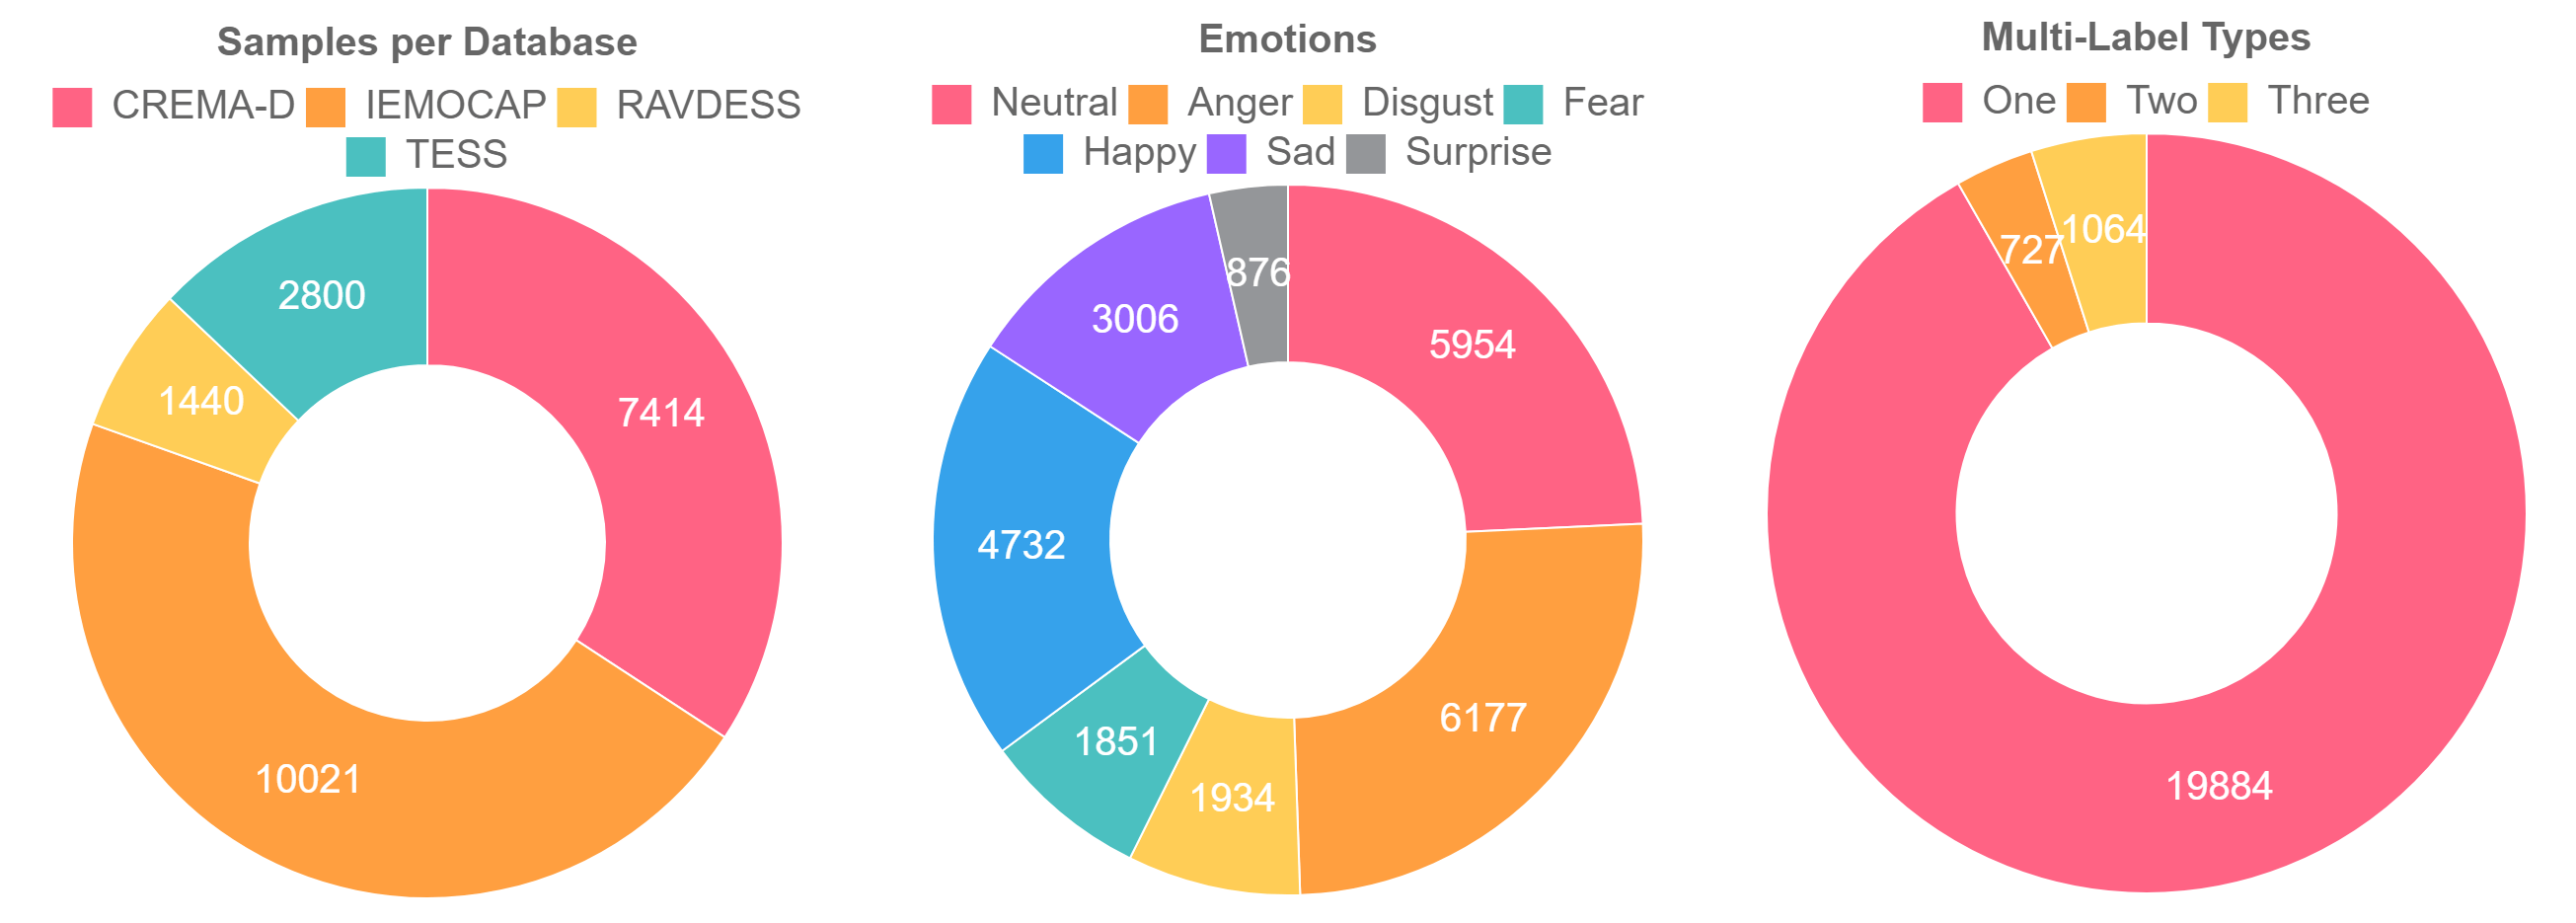
\includegraphics[width=\textwidth]{combined_db.png} 
	\caption{Proportions of each: database, emotion, and label types in the combined database.}
	\label{fig:combined_db}
\end{figure*}

Each sample from a database would flow through the same preprocessing steps to maintain consistency across all samples. A high level overview of the preprocessing steps is shown in figure \ref{fig:high_level_dataflow_diagram} and the detailed steps are described below.
\begin{enumerate}
	\item A sample starts as a raw waveform in the form of time series points specifying the amplitude at a certain point in time.
	\item The sample is then padded or cropped to the desired length of 4.5s. Shorter samples were zero-padded on the right tail. Longer samples were cropped and the extra information discarded.
	\item If the sample came from a database that we considered noisy, then a noise reduction filter was applied to the sample. We consider the IEMOCAP and CREMA-D databases to be noisy.
	\item The sample is then converted into a log-Mel spectrogram using the short-time Fourier transform (STFT) and Mel scale equation. The phase information was discard as it does not seem to hold relevant information. \cite{Kozakowski2017}
	\item The final step is to normalize the spectrograms to have values between negative one and one. This was done by using a minmax scaling function.
\end{enumerate}

For the STFT, we used a window size of 3072 with a 75\% overlap. For the Mel spectrogram, we set the minimum frequency to 20 Hz and maximum frequency to 12 kHz with 200 Mel bins.

\begin{figure}[]
	\centering
	\hspace{6mm}
	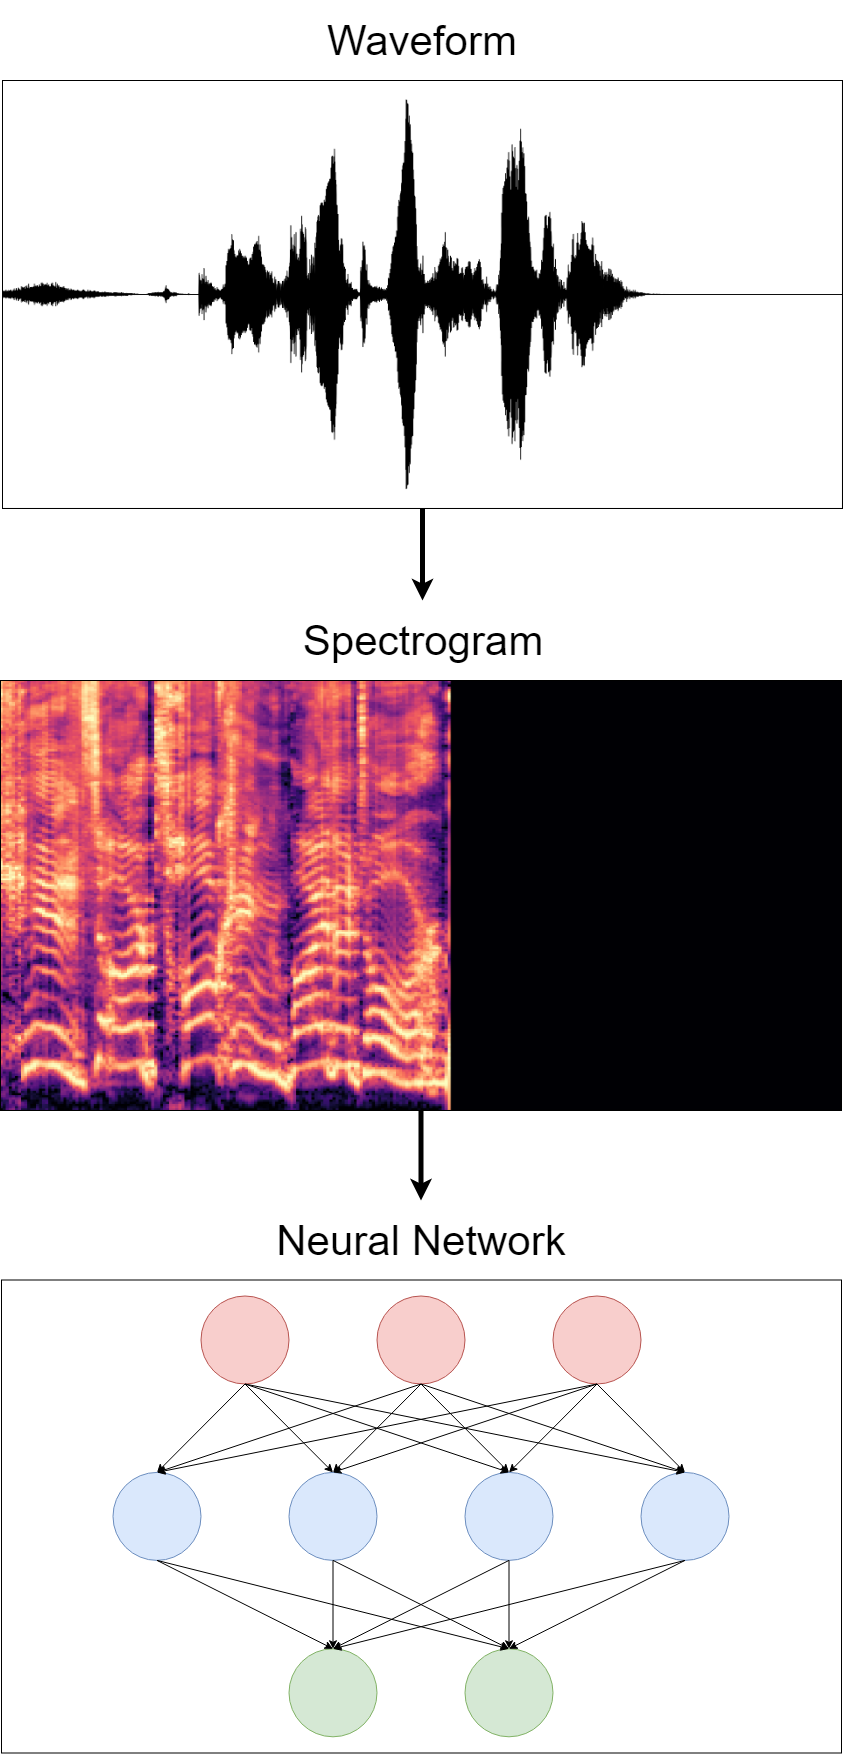
\includegraphics[width=\linewidth]{high_level_dataflow_diagram.png}
	\caption{A high level overview of the processing stages that a speech sample goes through.}
	\label{fig:high_level_dataflow_diagram}
\end{figure}

\subsection{Neural Network}

\begin{figure*}[b!]
	\centering
	\hspace{6mm}
	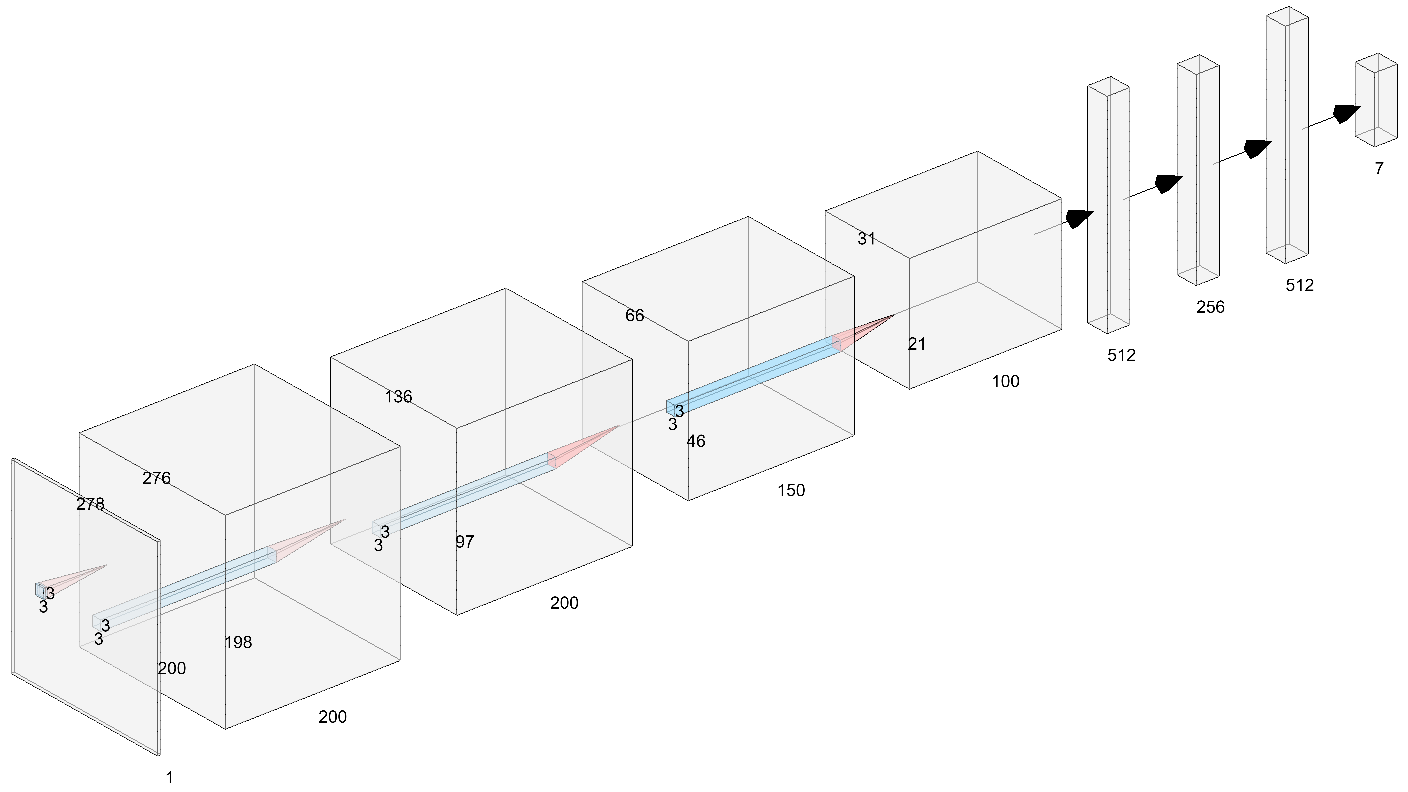
\includegraphics[width=\textwidth]{neural_network_architecture.png}
	\caption{Architecture for the speech emotion recognition network including the input layer and seven processing layers.}
	\label{fig:neural_network_architecture}
\end{figure*}

After all of the databases were processed this way, the final combined database was fed into a neural network for training, validation, and testing. We constructed a seven layer neural network consisting of four convolutional layers and three dense layers. The network architecture is shown in figure \ref{fig:neural_network_architecture}. The training process is described below.
\begin{itemize}
	\item We shuffled the combined database to make each input batch more uniform thus mitigating large gradient updates.
	\item We split the combined database into 80\% training, 10\% validation, and 10\% testing.
	\item We applied dropout \cite{Srivastava2014} to the dense layers and batch normalization \cite{Ioffe2015} to the convolutional layers to deal with overfitting.
	\item We updated the model's hyperparameters based on the validation loss and accuracy to improve the model's accuracy and ability to generalize.
	\item We used class weights during training to address class imbalance.
\end{itemize}

Table \ref{tab:model_hyperparams} describes the network hyperparameters and table \ref{tab:train_hyperparams} describes the training hyperparameters.

\begin{table}[b]
	\resizebox{\linewidth}{!}{%
		\begin{tabular}{|l|r|}
			\hline
			\textbf{Hyperparameter} & \textbf{Value} \\ \hline
			\rowcolor[HTML]{F6F8FA} 
			Input Dimensions & 278w x 200h x 1d \\ \hline
			Optimization Algorithm & Adam \\ \hline
			\rowcolor[HTML]{F6F8FA} 
			Loss Measure & Binary Cross-entropy \\ \hline
			Accuracy Metric & Categorical Cross-entropy \\ \hline
			\rowcolor[HTML]{F6F8FA} 
			Activation Function & Sigmoid \\ \hline
		\end{tabular}%
	}
	\caption{The model's hyperparameters.}
	\label{tab:model_hyperparams}
\end{table}

\begin{table}[]
	\resizebox{\linewidth}{!}{%
		\begin{tabular}{|l|r|}
			\hline
			\textbf{Hyperparameter} & \textbf{Value} \\ \hline
			\rowcolor[HTML]{F6F8FA} 
			Epochs & 20 \\ \hline
			Batch Size & 32 \\ \hline
			\rowcolor[HTML]{F6F8FA} 
			Training Set & 17,341 \\ \hline
			Validation Set & 2,167 \\ \hline
			\rowcolor[HTML]{F6F8FA} 
			Testing Set & 2,167 \\ \hline
		\end{tabular}%
	}
	\caption{The training hyperparameters.}
	\label{tab:train_hyperparams}
\end{table}

\section{Results}

After training the model, the model was evaluated on the testing set to get the final accuracy of the model. The final accuracy achieved was 52.57\%. Confusion matrices for each emotion are shown in Figure \ref{fig:confusion_matrix}.

\begin{figure}[]
	\centering
	\hspace{6mm}
	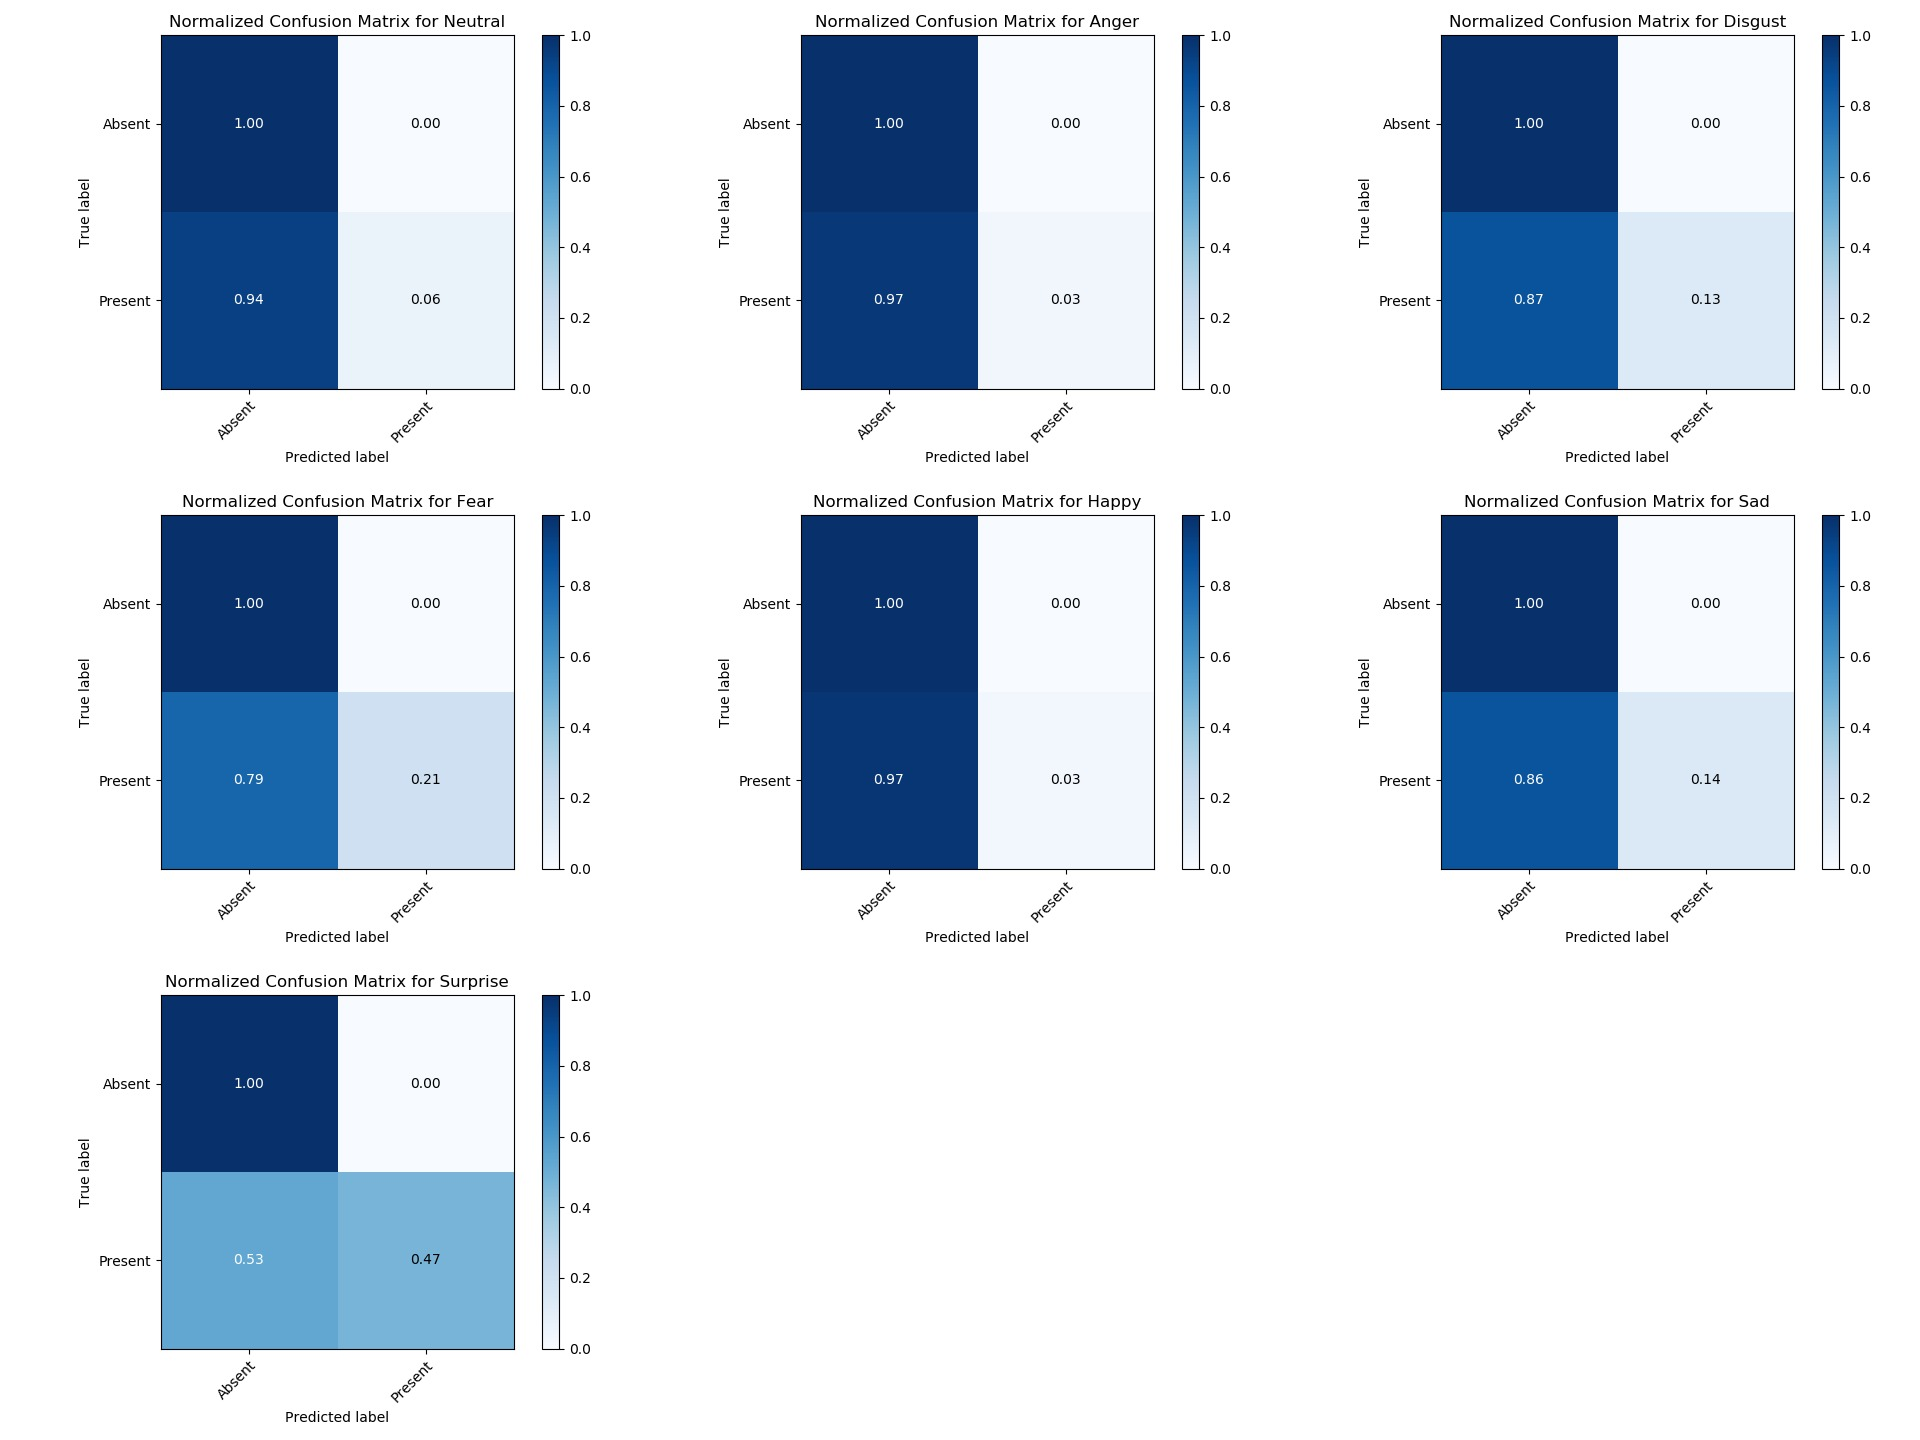
\includegraphics[width=\textwidth]{confusion_matrix.png}
	\caption{Confusion matrices for each emotion.}
	\label{fig:confusion_matrix}
\end{figure}

\section{Discussion}

We created a neural network model that achieved a classification accuracy of 52.57\% on the problem of multi-label emotion classification. This model can successfully classify multiple emotions in a sample and while this is a good result, we can do better.

\subsection{Limitations and Future Work}

One limitation of this work was that we only accounted for seven emotions but we know that there are more emotions than this. \cite{} Another limitations was that 
Here we present future improvements of our work 
\begin{itemize}
	\item Improving the recognition accuracy by using more sophisticated neural network architectures such as LSTMs or using more databases.
	\item Incorporating the phase data from the STFT and testing to see if that improves the accuracy.
	\item Testing a binary relevant approach to this multi-label problem and comparing it to this model.
\end{itemize}

\subsection{Conclusion}

Overall, this paper presented a convolutional neural network model that achieves a 52.57\% accuracy on multi-class, multi-label speech emotion recognition using four combined databases. We obtained this result by transforming raw speech samples into log-Mel spectrograms using STFT and the Mel scale. These log-Mel spectrograms are then fed into a eight layer neural network for classification for training. When we have completed training the neural network, the model was evaluated and achieved as 52.57\% accuracy. While this result is a promising start, we suggest improvements that future work can build upon to improve the accuracy.

\section*{Acknowledgment}
Acknowledge PURE award.


\bibliographystyle{IEEEtran}
\bibliography{IEEEabrv,references}

\end{document}
